\definecolor{exxetagray}{gray}{0.75}
\definecolor{itemcolor}{RGB}{179,217,255}
\definecolor{usercolor}{RGB}{255,204,179}

\shorthandoff{"}
\chapter{Multi-kriterielle Optimierung}
\label{ch:erweiterungen}
% Hier Überleitung finden zu Multi-kriterieller Optimierung in RS (Anknüpfen über Nutzen, der sich aus mehreren Aspekten zusammensetzt (hier: Nutzen setzt sich zusammen aus Präferenzen Manager und Präferenzen Mitarbeiter)).
% Grundsätzlich basiert das Rating eines Elements auf einem Kriterium.
Im vorangegangenen Kapitel wurde erläutert, dass für reziproke Empfehlungen sowohl die Präferenzen der Nutzer als auch die Präferenzen der Elemente berücksichtigt werden müssen.
% Irgendwo noch einbringen, dass Paarung quasi den Nutzen angibt, also gutes paar = guter Nutzen
Nach \textcite[S. 36]{li:inproceedings} ist eine optimale Paarung von Nutzer und Element demnach abhängig von zwei Attributen: der Bedürfniserfüllung des Empfehlungsempfängers und der Bedürfniserfüllung der empfohlenen Person.
Eine alleinige Betrachtung der Relevanz eines Elements für einen Nutzer (d.h. des Ratings) reicht in \ac{RRS} folglich nicht aus.
Für die Ermittlung des Nutzen einer \ac{N-E-K} in wechselseitigen Empfehlungssystemen müssen demnach mehrere Kriterien berücksichtigt werden.
% Die Kernfrage ist also: wie kann das Rating berechnet werden, wenn die Präferenzen von Elementen einbezogen werden sollen?
% Auch: Wie Gesamtrating ermitteln, wenn mehrere Kriterien berücksichtigt werden sollen? Wie sind Präferenzen zu gewichten? % S. 5, file:///C:/Users/masc6/Downloads/79_HDIOUD.pdf

\section{Einführung}
\label{ch:erweiterungen:einführung}
In den meisten Empfehlungssystemen erfolgt die Ermittlung des Nutzen einer \ac{N-E-K} anhand eines Kriteriums (z.B. der Gesamtbewertung eines Elements, Vgl. Kapitel \ref{ch:empfehlungssysteme:empfehlungserstellung:recommendation}) \cite[S. 847]{adomavicius:4:inbook}\cite[S. 745]{adomavicius:inproceedings}\cite[S. 49]{adomavicius:inproceedings:2}\cite[S. 424]{manouselis:article}\cite[S. 65]{lakiotaki:article}.
Nach \textcite[S. 847f.]{adomavicius:4:inbook} ist diese Annahme in der Literaur zuletzt in Teilen als unzureichend bezeichnet worden.
Es wird davon ausgegangen, dass der Nutzen eines Elements für einen Nutzer durchaus von mehreren Kriterien abhängen kann \cite[S. 847f.]{adomavicius:4:inbook}\cite[S. 424]{manouselis:article}.

In der Praxis existiert auch außerhalb des Bereichs der Empfehlungssysteme eine Vielzahl an Problemstellungen, für die unter der Berücksichtigung von oftmals konkurrierenden Kriterien eine optimale Lösung gefunden werden muss.
So zählt nach \textcite[S. ix]{statnikov:book} die Mehrheit aller Probleme der Ingenieurswissenschaft zu multi-kriteriellen Problemen.
Auch in anderen Bereichen wie dem Gesundheitswesen \cite[S. 195]{nemeth:article} oder der Marktforschung \cite[S. 50]{adomavicius:inproceedings:2} treten multi-kriterielle Probleme auf.
Ansätze für die Lösung solcher multi-kriteriellen Probleme werden allgemein unter dem Begriff der multi-kriteriellen Optimierung (engl.: multicriteria optimization) zusammengefasst \cite[S. v]{ehrgott:book}\cite[S. 867]{adomavicius:4:inbook}.
Zu bekannten Methoden zählen das Finden Pareto-Optimaler Lösungen \cite[S. 50]{adomavicius:inproceedings:2} und das Anwenden von Linearkombinationen zur Reduktion multi-kriterieller auf unikriterielle Probleme \cite[S. 745]{adomavicius:inproceedings}.

In der Entscheidungstheorie wird die Entscheidungsfindung in Organisationen ebenfalls als ein multi-kriterielles Problem behandelt, wobei verschiedene Aspekte wie Personal, Finanzen und Umwelt berücksichtigt werden müssen \cite[S. 50]{adomavicius:inproceedings:2}.
Ansätze, um Verantwortliche in dem Treffen von Entscheidungen anhand von (konkurrierenden) Kriterien zu unterstützen, werden gemäß \textcite[S. 50]{adomavicius:inproceedings:2} unter dem Begriff der multi-kriteriellen Entscheidungsunterstützung (engl.: \ac{MCDA}) zusammengefasst.
Outranking-Methoden zählen zu den bekanntesten Ansätzen in \ac{MCDA} \cite[S. 50]{adomavicius:inproceedings:2}.
Diese Ansätze ermöglichen es, Alternativen anhand unterschiedlicher Kriterien durch paarweise Vergleiche in Präferenz-Relation zu setzen \cite[S. 249]{bouyssou:inbook}.

Eine entscheidende Rolle in \ac{MCDA} spielt die Gewichtung der einzelnen Kriterien \cite[S. 206]{hdioud:inproceedings}\cite[S. 195]{nemeth:article}.
% Kriterien-Gewichte können entweder manuell festgelegt, oder unter dem Einsatz einer Gewicht\-ungs-Methode bestimmt werden \cite[S. 1]{vinogradova:article}.
% Das manuelle Festlegen von Gewichten umfasst Methoden, in denen Gewichte über Angaben von Stakeholdern zur Wichtigkeit der jeweiligen Kriterien bestimmt werden \cite[S. 196]{nemeth:article}.

% Wichtig ist hier eigentlich, dass die methoden noch nicht personalisiert sind, also immer nutzerübergreifend (was für uns ja eigentlich gut ist), siehe: file://wsl%24/Ubuntu/home/masc6/Projects/masterarbeit/literatur/New_Recommendation_Techniques_for_Multicriteria_Rating_Systems.pdf S. 50

\section{Bedeutung in Empfehlungssystemen}
Aus Sicht der Entscheidungstheorie \cite[S. 77]{jannach:inproceedings} können Empfehlungssysteme als entscheidungsunterstüztende Systeme verstanden werden \cite[S. 398f.]{huang:article}.
Demnach unterstützen Empfehlungssysteme die Nutzer eines Systems darin, aus einer Menge an Alternativen basierend auf mehreren Kriterien nützliche Elemente zu finden \cite[S. 398f.]{huang:article}.

Im Kontext von Empfehlungssystemen wurde der Einsatz von \ac{MCDA}-Metho\-den bereits in einigen Veröffentlichungen behandelt (siehe \cite{hdioud:inproceedings}\cite{zheng:inproceedings}\cite{adomavicius:4:inbook}\cite{adomavicius:inproceedings:2}).
\textcite[S. 849]{adomavicius:4:inbook} gehen davon aus, dass aufgrund der Generalität des Begriffs "multi-kriteriell", der multi-kriterielle Charakter \cite[S. 10]{adomavicius:5:inbook} der meisten Empfehlungssysteme auf unterschiedliche Grundideen verweisen kann.
Größtenteils können diese einer der folgenden Kategorien zugeordnet werden \cite[S. 10]{adomavicius:5:inbook}\cite[S. 849]{adomavicius:4:inbook}:
\begin{itemize}
    \item Multi-attribut-basierte Inhaltssuche, Filtern und Präferenzmodellierung
    \item Multi-objektive Empfehlungsstrategien
    \item Multi-kriterielle Bewertungen in der Präferenzerhebungen
\end{itemize}

Multi-attribut-basierte Inhaltssuche und multi-attribut-basiertes Filtern bezeichnen Systeme, die einem Nutzer ermöglichen seine Präferenzen unter Anwendung von Such- bzw. Filterprozessen spezifizieren \cite[S. 10]{adomavicius:5:inbook}\cite[S. 851]{adomavicius:4:inbook}.
Diese zusätzlichen Präferenzen können in solchen Systemen verwendet werden, um die Menge an potenziell nützlichen Elementen für einen Nutzer weiter einzugrenzen \cite[S. 11]{adomavicius:5:inbook}.
Unter multi-attribut-basierter Präferenzmodellierung wird die Darstellung von Präferenzen anhand verschiedener Attribute eines Elements verstanden (z.b. in klassischen inhaltsbasierten \ac{RS} \cite[S. 205]{hdioud:inproceedings}) \cite[S. 10]{adomavicius:5:inbook}.
Nach \textcite[S. 850]{adomavicius:4:inbook} werden diese Arten der multi-kriteriellen Empfehlung bereits durch existierende Typen von Empfehlungssystemen unterstützt (z.B. wissenbasierten, inhaltsbasierten und hybriden \ac{RS}).
% In hybriden Empfehlungssystemen können beispielsweise Bewertungen unterschiedlicher Algorithmen über eine Linearkombination zu einem Wert kombiniert werden \cite[S. 339]{burke:article}.
Ein Beispiel stellen Conversational \ac{RS} dar, die Präferenzen eines Nutzers neben Bewertungen über aktuelle Konversationen mit einem Nutzer (z.B. in Form eines Chatbots) erschließen \cite[S. 1]{yueming:article}.
% Hier beispiel einfügen? S. 4, https://iopscience.iop.org/article/10.1088/1742-6596/930/1/012050/pdf

Als multi-objektive Empfehlungsstrategien werden Implementierungen von Empfehlungssystemen verstanden, die für die Empfehlung von Elementen für einen Nutzer mehrere Ziele (engl.: Objectives) berücksichtigen \cite[S. 850]{adomavicius:4:inbook}.
Gemäß \textcite[S. 1097]{mcnee:inproceedings} verfolgen Empfehlungssysteme in der Literatur häufig ein Ziel, nämlich die Genauigkeit (engl.: Accuracy) der empfohlenen Elemente an einen Nutzer zu erhöhen.
Unter der Genauigkeit von Empfehlungen wird die Übereinstimmung einer vorhergesagten Bewertung durch das System mit der tatsächlichen Bewertung eines Nutzers verstanden \cite[S. 1098]{mcnee:inproceedings}.
In der Literatur wird davon ausgegangen, dass die Genauigkeit von Empfehlungen nicht immer ein alleiniger Indikator des tatsächlichen Nutzen von Empfehlungen ist \cite[S. 1097]{mcnee:inproceedings}\cite[S. 850]{adomavicius:4:inbook}\cite[S. 896]{adomavicius:article}.
Neben der Genauigkeit von Empfehlungen versuchen moderne Empfehlungssysteme daher oftmals die eingesetzten Algorithmen hinsichtlich weiterer Ziele (z.B. Diversität von Elementen \cite[S. 896]{adomavicius:article}, Serendipity \cite[S. 1099]{mcnee:inproceedings}) zu optimieren \cite[S. 850]{adomavicius:4:inbook}.
Multi-kriteriell bedeutet in solchen Systemen folglich die Empfehlungen für Nutzer unter Berücksichtigung mehrerer Ziele zu generieren \cite[S. 850]{adomavicius:4:inbook}.
% Beispiel?

Wird in der Literatur von multi-kriteriellen Empfehlungssystemen (engl.: \ac{MCRS}) gesprochen, wird sich zumeist auf multi-kriterielle Bewertungen in der Präferenzerhebung bezogen \cite[S. 207]{hdioud:inproceedings}\cite[S. 1156]{gupta:inproceedings}\cite[S. 327]{hassan:inproceedings}.
Während traditionelle Empfehlungssysteme Elemente anhand eines einzigen Kriteriums (z.b. der Gesamtbewertung) bewerten, werden Elemente in \ac{MCRS} anhand mehrerer Kriterien evaluiert \cite[S. 850]{adomavicius:4:inbook}\cite[S. 2]{adomavicius:5:inbook}.
Diese multi-kriteriellen Bewertungen werden häufig in Empfehlungssystemen des kollaborativen Filterns genutzt, um komplexe Präferenzen von Nutzern abzubilden \cite[S. 850]{adomavicius:4:inbook}.
Es wird davon ausgegangen, dass diese zusätzliche Information \cite[S. 49]{adomavicius:inproceedings:2} über die Präferenzen der Nutzer die Qualität der Empfehlungen verbessern kann \cite[S. 2]{adomavicius:5:inbook}.
Im Vergleich zu multi-attribut-basierten Grundideen werden für multi-kriterielle Bewertungen keine allgemeinen Präferenzen oder Gewichte für bestimmte Attribute durch einen Nutzer angegeben \cite[S. 851]{adomavicius:4:inbook}.

% Multi-kriterielle Probleme können in Empfehlungssystemen folglich in unterschiedlichen Kontexten bestehen.
% Aufgrund eines anhaltenden Trends im Bereich der multi-kriteriellen Bewertungen, beziehen sich die meisten Veröffentlichungen zu multi-kriteriellen Empfehlungssystemen in der Literatur auf multi-kriterielle Ratings.
% Daher werden Ansätze zur Lösung multi-kriterieller Optimierungsprobleme in Empfehlungssystemen Nachfolgend werden multi-kriterielle Empfehlungssysteme im Detail betrachtet und Lösungsansätze vorgestellt.

Multi-kriterielle Bewertungen in \ac{MCRS} werden wie unikriterielle Bewertungen in traditionellen Systemen über eine Rating-Funktion $R$ abgebildet.
Werden Elemente zusätzlich zu einer Gesamtbewertung anhand weiterer Kriterien bewertet, ergibt sich für die Rating-Funktion $R$ aus Gleichung \ref{eq10} \cite[S. 853]{adomavicius:4:inbook}:
\begin{equation}\label{eq11}
    R: Nutzer \times Element \rightarrow R_{0} \times R_{1} \times ... \times R_{k}
\end{equation}
Hierbei stellt $R_{0}$ die Menge aller möglichen Gesamtbewertungen dar.\footnote{Da aus Gründen der Einfachheit in Kapitel \ref{ch:empfehlungssysteme:nutzenfunktion} für den Nutzen einer \ac{N-E-K} die Bewertung eines Nutzers für ein Element angenommen wurde, entspricht $R_{0}$ dem $Rating$ (Vgl. Gleichung \ref{eq2} und \ref{eq10}).}
$R_{i}$ bildet die Menge aller möglichen Bewertungen jedes einzelnen Kriteriums $i$ ($i=1,...,k$) ab \cite[S. 49]{adomavicius:inproceedings:2}.

Bilden \ac{MCRS} lediglich die Bewertungen der einzelnen Kriterien ab, ergibt sich für die Rating-Funktion $R$ folgende Form \cite[S. 853]{adomavicius:4:inbook}:
\begin{equation}\label{eq12}
    R: Nutzer \times Element \rightarrow R_{1} \times ... \times R_{k}
\end{equation}

Tabelle \ref{tab3} bildet beispielhaft multi-kriterielle Bewertungen von Mitarbeitern eines Unternehmens für Fähigkeiten ab.
Hierbei setzt sich eine Gesamtbewertung aus dem Kenntnisstand eines Mitarbeiters und dessen Präferenzen für eine Fähigkeit zusammen.

\begin{table}[htbp]
    \begin{center}
    \begin{tabular}{|c||c|c|c|}
    \hline
    {} & {\textbf{Java}} & {\textbf{Python}} & {\textbf{MySQL}}\\
    \hline
    \hline
    \textbf{Jane D.} & $2_{0,2}$ & $4_{3,1}$ & $2_{0,2}$ \\
    \hline
    \textbf{John D.} & $2_{1,1}$ & $4_{1,3}$ & ? \\
    \hline
    \textbf{Max M.} & $3_{2,1}$ & $3_{1,2}$ & $3_{2,1}$ \\
    \hline
    \end{tabular}
    \end{center}
    \caption[Multi-kriterielle Rating-Matrix ]{Multi-kriterielle Rating-Matrix \\
    (Eigene Darstellung in Anlehnung an \cite[S. 51]{adomavicius:inproceedings:2})}
	\label{tab3}
\end{table}

Eine alleinige Betrachtung der Gesamtbewertungen von Mitarbeitern lässt vermuten, dass der Mitarbeiter John D. am meisten Ähnlichkeit mit der Mitarbeiterin Jane D. aufweist.
Basierend auf den multi-kriteriellen Bewertungen scheint der Mitarbeiter Max M. jedoch mehr Ähnlichkeit mit John D. aufzuweisen als die Mitarbeiterin Jane D.
Es wird deutlich, dass durch die Abbildung des Nutzen eines Mitarbeiters über ein einziges Kriterium, Unterschiede bzw. Gemeinsamkeiten zwischen Nutzern unentdeckt bleiben können \cite[S. 854]{adomavicius:4:inbook}.
Durch die multi-kriteriellen Bewertungen können zusätzliche Information über die Präferenzen der Mitarbeiter des Systems abgebildet werden.
Diese können wiederum für die Vorhersage fehlender Transaktionen genutzt werden (z.B. Vorhersage von $\hat{r}_{John D., MySQL}$ anhand der Ähnlichkeit zu Max M.) \cite[S. 848]{adomavicius:4:inbook}.

Multi-kriterielle Optimierungsprobleme können in Empfehlungssystemen folglich in unterschiedlichen Kontexten bestehen.
Aufgrund eines anhaltenden Trends im Bereich der multi-kriteriellen Bewertungen \cite[S. 851]{adomavicius:4:inbook}, beziehen sich die meisten Veröffentlichungen zu Lösungsansätzen multi-kriteriel\-ler Optimierungsprobleme in der Literatur auf multi-kriterielle Ratings.
Auch wenn der Kontext der multi-kriteriellen Probleme sich unterscheiden kann, können viele Lösungsansätze in allen Bereichen eingesetzt werden.
Daher werden nachfolgend Lösungsansätze multi-kriterieller Optimierungsprobleme am Beispiel multi-kriterieller Bewertungen angeführt.

% \section{Problemstellung}

\section{Lösungsansätze}
Nach \textcite[S. 853]{adomavicius:4:inbook} stellt die Integration multi-kriteriel\-ler Bewertungen in bestehende Techniken eine der wichtigsten Themen zukünftiger Empfehlungssysteme dar.
In der Literatur existieren bereits einige Veröffentlichungen, die grundlegende Techniken zur Integration multi-kriterieller Bewertungen in Empfehlungssysteme betrachten (siehe \cite{recommenderSystems:2016}\cite{adomavicius:4:inbook}\cite{adomavicius:inproceedings:2}).
Abhängig davon, in welcher Phase des Empfehlungserstellungsprozesses die Techniken eingesetzt werden, werden diese in der Literatur einer von zwei Kategorien zugeordnet: Einsatz multi-kriterieller Bewertungen in der Vorhersage oder Einsatz multi-kriterieller Bewertungen im Ranking \cite[S. 854]{adomavicius:4:inbook}.

Während der Vorhersage-Phase können multi-kriterielle Bewertungen eingesetzt werden, um Gesamtbewertungen bzw. Bewertungen individueller Kriterien vorherzusagen \cite[S. 854]{adomavicius:4:inbook}.
Häufig werden multi-kriterielle Bewertungen für die Vorhersage in Systemen des kollaborativen Filterns verwendet \cite[S. 850]{adomavicius:4:inbook}.
Traditionell werden Techniken für die Vorhersage in Systemen des kollaborativen Filterns in modellbasierte und speicherbasierte Techniken unterschieden.
Modellbasierte Techniken verwenden Methoden der Statistik und des Maschinellen Lernens, um basierend auf historischen Daten Modelle zu entwickeln, über die fehlende Transaktionen vorhergesagt werden können.
Im Gegensatz dazu ermitteln speicherbasierte Systeme Vorhersagen "on the fly" \cite[S. 855]{adomavicius:4:inbook} basierend auf aktuell vorliegenden Daten.
Für die Vorhersage werden heuristische Methoden verwendet \cite[S. 855]{adomavicius:4:inbook}.
% Wie komme ich hier darum herum so ins detail der techniken von nachbarschaftsbasierten algorithmen zu gehen?
Abhängig davon, welche Technik für die Vorhersage angewandt wird, unterscheiden sich Lösungsansätze multi-kriterieller Bewertungen in der Vorhersage weiter in speicherbasierte- und modellbasierte Ansätze.

\subsection{Speicherbasierte Ansätze}
In speicherbasierten Systemen des kollaborativen Filterns erfolgt die Vorhersage fehlender Bewertungen grundsätzlich durch Aggregation \cite[S.738]{adomavicius:inproceedings} von Bewertungen ähnlicher Nutzer bzw. ähnlicher Elemente.
Dies basiert auf der Annahme, dass ähnliche Nutzer ähnliches Bewertungsverhalten aufweisen (nutzerbasiertes kollaboratives Filtern) bzw. ähnliche Elemente ähnliche Bewertungen erhalten (elementbasiertes kollaboratives Filtern) \cite[S. 29]{recommenderSystems:2016}.
In der Praxis verwenden die meisten Systeme des kollaborativen Filterns Ähnlichkeiten zwischen Nutzern für die Vorhersage fehlender Bewertungen \cite[S. 427]{recommenderSystems:2016}.
Eine Vorhersage stellt demnach eine Aggregation der Bewertungen eines Zielelements durch Nutzer dar, die (basiernd auf ihren vorherigen Bewertungen) Ähnlichkeit zu einem Zielnutzer aufweisen \cite[S.738]{adomavicius:inproceedings}.

Für die Ermittlung der Ähnlichkeit $sim(c,c')$ zweier Nutzer $c$ und $c'$, können verschiedene Ähnlichkeitsmaße herangezogen werden.
Zu den bekanntesten paarweisen Ähnlichkeitsmaßen zählen der Pearson-Korrelationskoeffizient und die Kosinus-Ähnlichkeit \cite[S. 856]{adomavicius:4:inbook}\cite[S. 738]{adomavicius:inproceedings}.
% Hier Maße mit reinnehmen oder nicht?
Angenommen $S(c,c')$ stellt die Menge aller Elemente aus $S$ dar, die beide Nutzer bewertet haben (d.h. $S(c,c')=\{s \in S | r_{cs} \neq ? \cap r_{c's} \neq ?\}$ \cite[S. 738]{adomavicius:inproceedings}), so werden die Ähnlichkeitsmaße wie folgt ermittelt \cite[S. 856]{adomavicius:4:inbook}:
\begin{itemize}
    \item Pearson-Korrelationskoeffizient:
    \begin{equation}\label{eq13}
        sim(c,c') = \frac{\sum\limits_{s \in S(c,c')}(r_{cs}-\overline{r(c)})(r_{c's}-\overline{r(c')})}{\sqrt{\sum\limits_{s \in S(c,c')}(r_{cs}-\overline{r(c)})^{2}}\sqrt{\sum\limits_{s \in S(c,c')}(r_{c's}-\overline{r(c')})^{2}}}
    \end{equation}
    \item Kosinus-Ähnlichkeit:
    \begin{equation}\label{eq14}
        sim(c,c') = \frac{\sum\limits_{s \in S(c,c')}r_{cs}r_{c's}}{\sqrt{\sum\limits_{s \in S(c,c')}r_{cs}^{2}}\sqrt{\sum\limits_{s \in S(c,c')}r_{c's}^{2}}}
    \end{equation}
\end{itemize}
Der Parameter $\overline{r(c)}$ repräsentiert die durchschnittliche Bewertung eines Nutzers $c$.

Gemäß \textcite[S. 856f.]{adomavicius:4:inbook} können Ähnlichkeitsmaße wie der Pearson-Korrelationskoeffizient oder die Kosinus-Ähnlichkeit lediglich Bewertungen anhand eines einzelnen Kriteriums verarbeiten.
In \ac{MCRS} besteht eine Bewertung $r$ jedoch neben einer Gesamtbewertung $r^{0}$ zusätzlich aus $k$ multi-kriteriellen Bewertungen $r^{1}, ..., r^{k}$, d.h. $r=(r^{0},r^{1}, ..., r^{k})$ \cite[S. 426]{recommenderSystems:2016}\cite[S. 857]{adomavicius:4:inbook}.
Anstelle eines einzigen Ratings besitzt eine \ac{N-E-K} in \ac{MCRS} demnach $k+1$ Bewertungen \cite[S. 857]{adomavicius:4:inbook}.\footnote{Für \ac{MCRS}, die keine Gesamtbewertungen beinhalten, können für die Berechnung der Ähnlichkeit dieselben Maße angewandt werden, wie für Systeme die Gesamtbewertungen verwenden, mit dem einzigen Unterschied, dass der Index $i$ nicht die Gesamtbewertung einschließt (d.h. $i \in \{1,k\}$ anstelle von $i \in \{0,k\}$) \cite[S. 857]{adomavicius:4:inbook}.}
Daher können multi-kriterielle Bewertungen nicht unmittelbar auf die Gleichungen angewandt werden.
In Anlehnung an \textcite[S. 49]{adomavicius:inproceedings:2}, \textcite[S. 860]{adomavicius:4:inbook} und \textcite[S. 427]{recommenderSystems:2016} wird die Vorstellung der Lösungsansätze auf nutzerbasiertes kollaboratives Filtern begrenzt.\footnote{Für ein simples Vorgehen zur Umstellung der Berechnungen auf elementbasiertes kollaboratives Filtern wird auf \textcite[S. 49]{adomavicius:inproceedings:2} verwiesen.}

Ein speicherbasierter Ansatz für die Berücksichtigung multi-kriterieller Bewertungen in der Ähnlichkeitsberechnung stellt die Aggregation von Ähnlichkeiten auf Ebene der einzelnen Kriterien dar.
Gibt $sim^{i}(c,c')$ die Ähnlichkeit zweier Nutzer $c$ und $c'$ für jedes Kriterium $i \in \{0,k\}$ an, so kann deren Ähnlichkeit nach \textcite[S. 427]{recommenderSystems:2016} allgemein wie folgt ermittelt werden:
\begin{enumerate}
    \item Berechnung der Ähnlichkeit $sim^{i}(c,c')$ für jedes Kriterium $i \in \{0,k\}$ anhand eines paarweisen Ähnlichkeitsmaßes (z.B. Pearson-Korrelations\-koeffizient, Kosinus-Ähnlichkeit).
    \item Berechnung der aggregierten Ähnlichkeit $sim^{aggr}(c,c')$ anhand einer Aggregations-Funktion über alle Ähnlichkeiten der einzlenen Kriterien:
    \begin{equation}
        sim^{aggr}(c,c') = F(sim^{0}(c,c'), sim^{1}(c,c'), ..., sim^{k}(c,c'))
    \end{equation}
\end{enumerate}

Nach \textcite[S. 427]{recommenderSystems:2016} und \textcite[S. 857]{adomavicius:4:inbook} zählen zu den bekanntesten Aggregations-Funktionen multi-kriterieller Bewertungen:
\begin{itemize}
    \item die durchschnittliche Ähnlichkeit:
    \begin{equation}\label{eq15}
        sim^{aggr}(c,c') = \frac{\sum\limits_{i=0}^{k}sim^{i}(c,c')}{k+1}
    \end{equation}
    \item die pessimistische Ähnlichkeit:
    \begin{equation}\label{eq16}
        sim^{aggr}(c,c') = \underset{i=0,...,k}{\min}\textnormal{ }sim^{i}(c,c')
    \end{equation}
    \item sowie die gewichtete Ähnlichkeit:
    \begin{equation}\label{eq17}
        sim^{aggr}(c,c') = \sum\limits_{i=0}^{k}w^{i}sim^{i}(c,c')
    \end{equation}
\end{itemize}

Die durchschnittliche Ähnlichkeit wird ermittelt, indem die Summe der Ähnlichkeiten der einzelnen Kriterien durch die Anzahl der Kriterien plus Gesamtbewertung $k+1$ geteilt wird.
Für die pessimistische Ähnlichkeit wird aus allen Ähnlichkeiten der einzelnen Kriterien (inkl. Gesamtbewertung) die kleinstse Ähnlichkeit bestimmt \cite[S. 427]{recommenderSystems:2016}.
Die gewichtete Ähnlichkeit multikriterieller Bewertungen \cite[Kapitel 6.1 The Algorithm, Abs. 1ff.]{tang:article} stellt eine Verallgemeinerung der durchschnittlichen Ähnlichkeit dar \cite[S. 427]{recommenderSystems:2016}.
Hierbei stellt $w^{i}$ das Gewicht des Kriteriums $i$ $(i=0,...,k)$ dar, welches nach \textcite[S. 857]{adomavicius:4:inbook} angibt, wie wichtig ein Kriterium für eine Empfehlung ist.
Die Werte der Gewichte können gemäß \textcite[S. 428]{recommenderSystems:2016} mithilfe herkömmlicher Parameteroptimierungs-Techniken (z.b. Kreuzvalidierung) bestimmt werden.

Neben der Ähnlichkeitsberechnung mit anschließender Aggregation kann die Ähnlichkeit zweier Nutzer unter Berücksichtigung multi-kriterieller Bewertungen auch über multidimensionale Distanzmaße ermittelt werden \cite[S. 857]{adomavicius:4:inbook}.
Für diesen speicherbasierten Ansatz wird im ersten Schritt die Ähnlichkeit zweier Nutzer $c$ und $c'$ basierend auf einem Element $s$ über ein herkömmliches Distanzmaß ermittelt.
% Hier Maße mit reinnehmen oder nicht?
Zu bekannten Distanzmaßen zählen \textcite[S. 857f.]{adomavicius:4:inbook}:
\begin{itemize}
    \item die Manhattan-Distanz:
    \begin{equation}\label{eq18}
        elementDist^{aggr}(c,c',s)= \sum\limits_{i=0}^{k}|r_{cs}^{i}-r_{c's}^{i}|
    \end{equation}
    \item sowie die Euklidische Distanz:
    \begin{equation}\label{eq19}
        elementDist^{aggr}(c,c',s)= \sqrt{\sum\limits_{i=0}^{k}(|r_{cs}^{i}-r_{c's}^{i}|)^{2}}
    \end{equation}
\end{itemize}

Nach \textcite[S. 240]{sahoo:article} berücksichtigen diese Distanzmaße nicht mögliche Abhängigkeiten (Korrelationen) zwischen den einzelnen Kriterien (inkl. Gesamtbewertung).
Abhängigkeit bedeutet, dass nicht jedes Bewertungskriterium gänzlich neue Information über die Präferenzen eines Nutzers liefert, sondern ein Kriterium stärkeren Einfluss auf die Ausprägung der Bewertungen der anderen Kriterien haben kann \cite[S. 235]{sahoo:article}.
Ein multidimensionales Distanzmaß, welches Abhängigkeiten zwischen Kriterien berücksichtigt ist die Mahalanobis-Distanz.
Dieses Maß ermittelt die Distanz zwischen zwei Vektoren $\vec{c}$ und $\vec{c'}$ unter Einbezug der Kovarianz-Matrix $V$:
\begin{equation}\label{eq25}
    elementDist^{aggr}(\vec{c},\vec{c'}) = \sqrt{(\vec{c}-\vec{c'})^{T}V^{-1}(\vec{c}-\vec{c'})}
\end{equation}
Hierbei stellt ein Vektor die muti-kriteriellen Bewertungen eines Elements $s$ durch einen Nutzer dar.
Die Kovarianz-Matrix ermitteln \textcite[S. 240]{sahoo:article} basierend auf historsichen Daten zu Bewertungen der Nutzer.

Die Gesamtdistanz zweier Nutzer $c$ und $c'$ wird, unabhängig von der Wahl des Distanzmaßes, als Durchschnitt über alle Elemente in $S(c,c')$ ermittelt, d.h. für alle Elemente, die beide Nutzer bewertet haben \cite[S. 858]{adomavicius:4:inbook}:
\begin{equation}\label{eq20}
    dist^{aggr}(c,c')= \frac{\sum\limits_{s \in S(c,c')}elementDist^{aggr}(c,c',s)}{|S(c,c')|}
\end{equation}

Aus der Gesamtdistanz lässt sich die Ähnlichkeit zweier Nutzer wie folgt ableiten \cite[S. 858]{adomavicius:4:inbook}:
\begin{equation}\label{eq21}
    sim^{aggr}(c,c') = \frac{1}{1 + dist^{aggr}(c,c')}
\end{equation}

Speicherbasierte Ansätze beeinflussen lediglich die Ähnlichkeitsberechnung in kollaborativen Systemen.\footnote{Die speicherbasierten Ansätze werden daher auch als ähnlichkeitsbasierte Ansätze bezeichnet \cite[S. 52]{adomavicius:inproceedings:2}.}
Das bedeutet, fehlende Bewertungen können nach Ermittlung der Ähnlichkeit wie gewohnt mittels Aggregation (z.B. gewichtete Summe \cite[S. 859]{adomavicius:4:inbook}) bestimmt werden \cite[S. 52]{adomavicius:inproceedings:2}\cite[S. 428]{recommenderSystems:2016}.

\subsection{Modellbasierte Ansätze}
Im Vergleich zu speicherbasierten Algorithmen des kollaborativen Filterns, werden fehlende Bewertungen in traditionellen modellbasierten Systemen über Vorhersage-Modelle bestimmt \cite[S. 861]{recommenderSystems:2016}.
Basierend auf vergangenen Bewertungen der Nutzer eines Systems \cite[S. 358]{jin:article}, werden diese Vorhersage-Modelle im Vorfeld entwickelt (bspw. anhand von statistischen Modellen) \cite[S. 71]{recommenderSystems:2016}.
In der Literatur existieren bereits einige Ansätze für die Integration multi-kriterieller Bewertungen in modellbasierte Systeme \cite[S. 861]{adomavicius:4:inbook}.

Nach \textcite[S. 861]{adomavicius:4:inbook} besteht ein Nachteil speicherbasierter Ansätze darin, dass sich deren Einsatz auf Systeme des kollaborativen Filterns beschränkt.
Ein alternativer Ansatz, der in Kombination mit jeglicher Art an Empfehlungssystem verwendet werden kann, stellt der Aggregation-Function-Ansatz von \textcite[S. 52ff.]{adomavicius:inproceedings:2} dar \cite[S. 861]{adomavicius:4:inbook}.
Dem Ansatz liegt die Idee zugrunde, dass Gesamtbewertungen von Elementen eine Kombination (Aggregation) ihrer zugehörigen multi-kriteriellen Bewertungen darstellen \cite[S. 861]{adomavicius:4:inbook}.
Gemäß \textcite[S. 52]{adomavicius:inproceedings:2} wird eine Gesamtbewertung $r^{0}$ durch eine Aggregationfunktion $f$ ihrer multikriteriellen Bewertungen $r^{1}, ..., r^{k}$ repräsentiert:
\begin{equation}\label{eq22}
    r^{0} = f(r^{1}, ..., r^{k})
\end{equation}
Das bedeutet, der Aggregation-Function-Ansatz unterstellt eine bestimmte Beziehung zwischen der Gesamtbewertung eines Elements durch einen Nutzer und dessen multi-kriterieller Bewertungen \cite[S. 52]{adomavicius:inproceedings:2}.
So kann es sein, dass die Präferenz von Mitarbeitern für Fähigkeiten eine stärkere Priorität besitzt, d.h. das die meisten Mitarbeiter Fähigkeiten tatsächlich hoch bewerten, wenn sie diese gleichzeitig präferieren (Vgl. Tabelle \ref{tab3}).
Nach dieser Annahme müsste eine hoch vorhergesagte Präferenz eines Mitarbeiters für eine Fähigkeit ebenfalls in einer hoch vorhergesagten Gesamtbewertung resultieren \cite[S. 52]{adomavicius:inproceedings:2}.

Die Vorhersage von Gesamtbewertungen nach dem Aggregation-Function-Ansatz erfolgt anhand von drei Schritten, welche nachfolgend in Abbildung \ref{fig:optimierung:loesungen:abb1} grafisch abgebildet sind.

\begin{figure}[H]
    \centering
	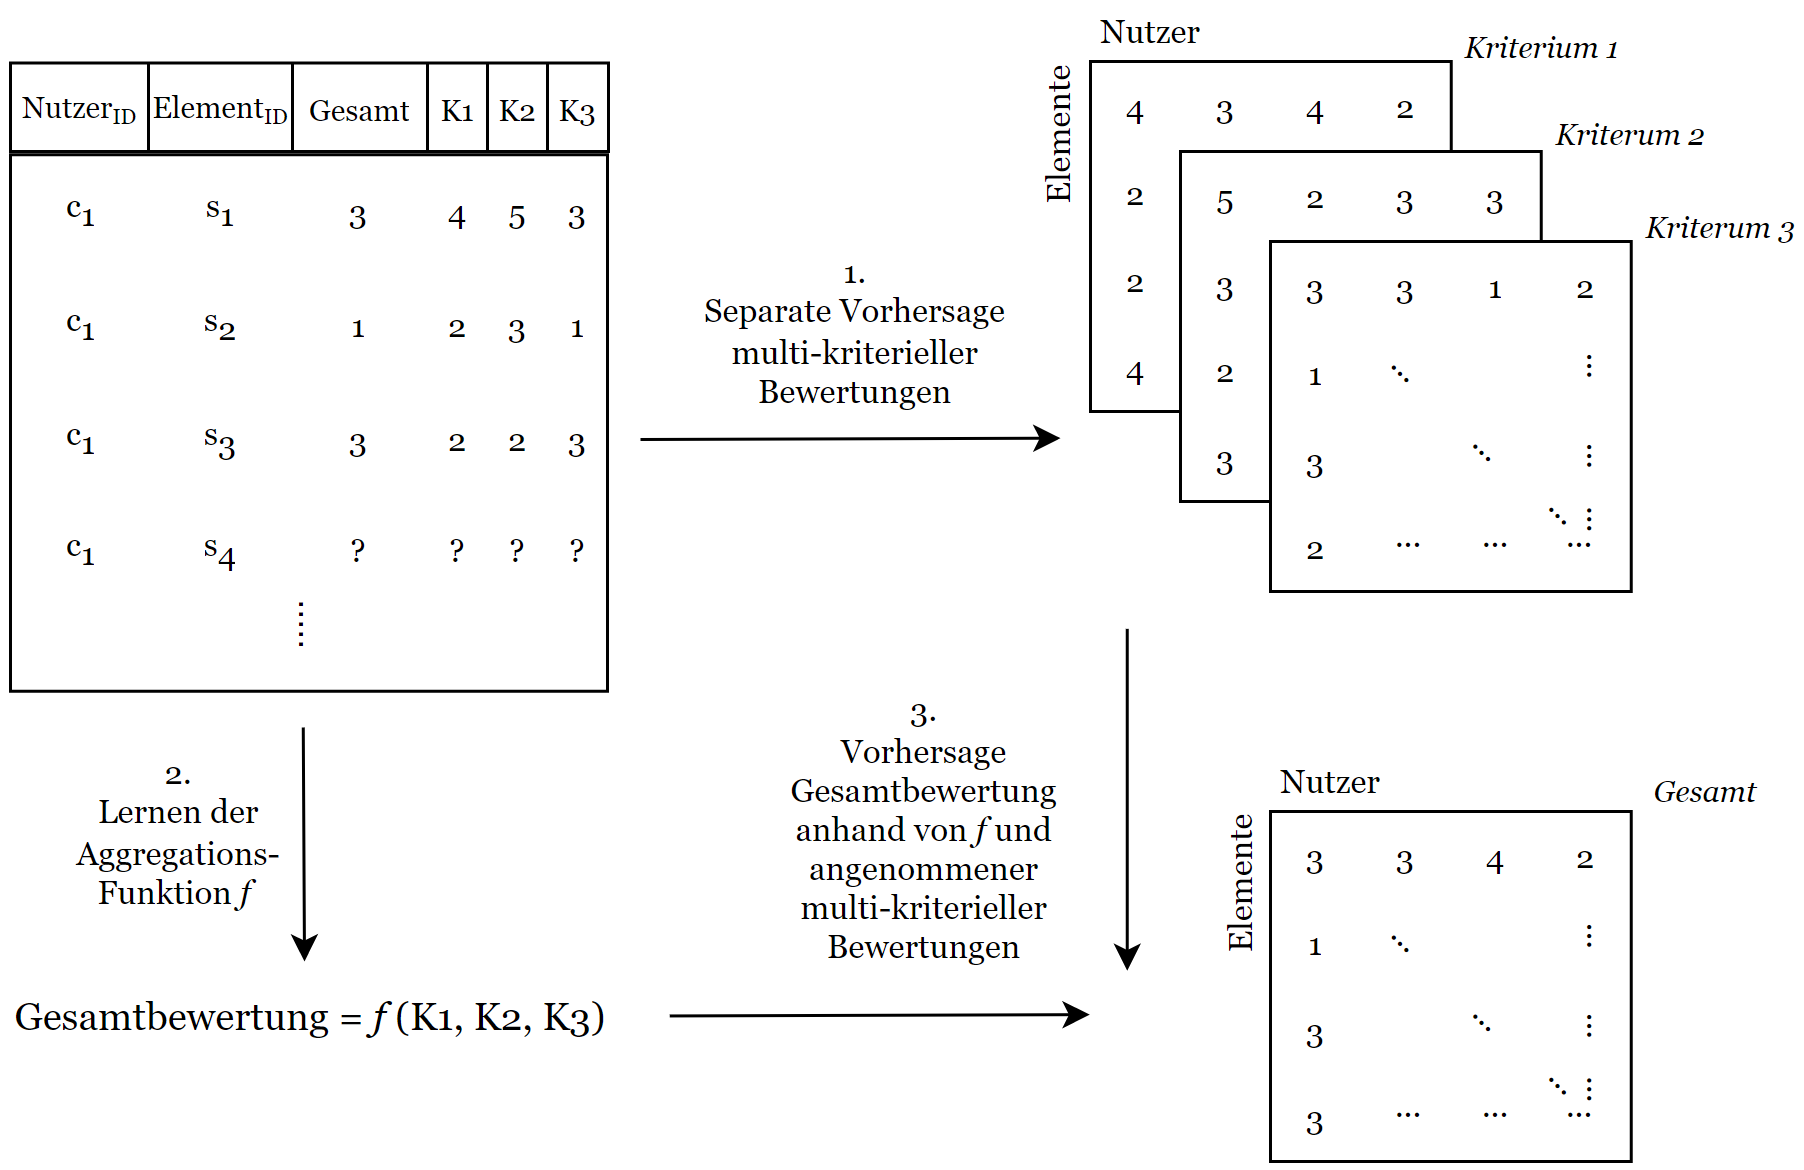
\includegraphics[width=1.0\textwidth]{gfx/a-f-ansatz.png}
	\caption[Aggregation-Function-Ansatz]{Aggregation-Function-Ansatz\\
    (Eigene Darstellung in Anlehnung an \cite[S. 862]{adomavicius:4:inbook})}
	\label{fig:optimierung:loesungen:abb1}
\end{figure}

Im ersten Schritt wird die $k$-dimensionale Rating-Matrix in $k$ unikriterielle Rating-Matrizen der traditionellen Form (Nutzer$\times$Element-Matrix) aufgeteilt \cite[S. 53]{adomavicius:inproceedings:2}.
Für jedes Kriterium $i \in {1,...,k}$ wird daraufhin unter Anwendung eines beliebigen Algorithmus (z.B.: kollaboratives Filtern, inhaltsbasierte Algorithmen) dessen fehlende Bewertungen vorhergesagt \cite[S. 428]{recommenderSystems:2016}.
Dadurch wird das $k$-dimensionale multi-kriterielle Problem in $k$ unikriterielle Probleme zerlegt \cite[S. 861]{adomavicius:4:inbook}.
Schritt 2 umfasst das Aufstellen der Aggregatios-Funktion $f$.
Nach \textcite[S. 53]{adomavicius:inproceedings:2} existieren hierfür maßgeblich drei Verfahren:
\begin{itemize}
    \item \textit{Domänenwissen:} Aufstellen der Funktion basierend auf Erfahrungen und Domänenwissen. Ein simpler Ansatz stellt der Durchschnitt aller angenommenen Bewertungen der einzelnen Kriterien als Aggregations-Funktion dar.
    \item \textit{Statistische Methoden:} Aufstellen der Funktion anhand statistischer Verfahren (z.B. lineare und nicht-lineare Regressionsanalysen) \cite[S. 53]{adomavicius:inproceedings:2}. So kann die Vorhersage einer Gesamtbewertung in der linearen Regression als eine Linearkombination der (angenommenen) multi-kriteriellen Bewertungen repräsentiert werden \cite[S. 429]{recommenderSystems:2016}:
    \begin{equation}\label{eq23}
        \hat{r}^{0} = \sum\limits_{i=1}^{k}w^{i} r^{i}
    \end{equation}
    Die Gewichte $w^{1}, ..., w^{k}$ der Kriterien können anhand verschiedener Techniken der linearen Regression bestimmt werden \cite[S. 429]{recommenderSystems:2016}.
    \item \textit{Techniken des Maschinellen Lernens:} Aufstellen der Funktion über Modelle des Maschinellen Lernens (z.B. neuronale Netze) \cite[S. 53]{adomavicius:inproceedings:2}.
\end{itemize}
Weiter unterscheiden \textcite[S. 53]{adomavicius:inproceedings:2} Aggregations-Funk\-tionen in Abhängigkeit ihres Bezugs.
Wird eine Funktion verwendet um Vorhersagen für alle \ac{N-E-K}-en übergreifend zu treffen, wird diese als total Aggregation-Function bezeichnet (d.h. Gewichte sind nutzer- bzw. elementübergreifend festgesetzt).
Als nutzerbasiert bzw. elementbasiert wird eine Aggregations-Funktion bezeichnet, die basierend auf Bewertungen eines einzelnen Nutzers bzw. Elements bestimmt wird.
Dies kann in Domänen sinnvoll sein, in denen sich die Gewichte einzelner Kriterien zwischen Nutzern bzw. Elementen stark unterscheiden \cite[S. 53]{adomavicius:inproceedings:2}.

Im letzten Schritt erfolgt die Vorhersage der Gesamtbewertungen basierend auf den (angenommenen) multi-kriteriellen Bewertungen und der erstellten Aggregation-Function $f$ \cite[S. 861]{adomavicius:4:inbook}.

Neben dem Aggregation-Function-Ansatz nennen \textcite[S. 861]{adomavicius:4:inbook} probabilistische Modellierungs-Ansätze für die Integration multi-kriterieller Bewertungen in Empfehlungssystemen.
Vereinfacht gesehen handelt es sich dabei um Methoden, die mit Wahrscheinlichkeiten für Bewertungen arbeiten.
\textcite[S. 861]{adomavicius:4:inbook} nennen als Beispiel die Veröffentlichung von \textcite[S. 231]{sahoo:article}.
In der Veröffentlichung wird eine Anpassung des \ac{FMM} von \textcite[S. 704ff.]{si:inproceedings} um multi-krierielle Bewertungen vorgestellt.
\textcite[S. 358]{jin:article} beschreiben das \ac{FMM} als eine grafische Darstellung eines probabilistischen Modells, in dem Nutzer und Elemente (mehreren)\footnote{Das \ac{FMM} unterscheidet sich von herkömmlichen grafischen Modellen unter anderem darin, dass Nutzer bzw. Elemente mehreren Clustern zugeordnet werden können \cite[S. 3]{si:inproceedings}\cite[S. 366]{jin:article}.} Clustern (Klassen) zugeordnet werden können.
Das \ac{FMM} folgt der Annahme, dass eine Bewertung r, welche ein Element s von einem Nutzer c erhält, von einer latenten Variable $Z_{c}$ und einer latenten Variable $Z_{s}$ abhängt \cite[S. 235]{sahoo:article}.
$Z_{c}$ kennzeichnet die Klasse(n), denen ein Nutzer $c$ und ${Z_{s}}$ die Klasse(n), denen ein Element $s$ zugeordnet werden kann \cite[S. 862]{adomavicius:4:inbook}\cite[S. 3]{si:inproceedings}.
Die Wahrscheinlichkeit der Bewertung $r$ eines Nutzers $c$ für ein Element $s$ ergibt sich nach \textcite[S. 862]{adomavicius:4:inbook} aus der Summe aller Wahrscheinlichkeiten der Kombinationen der Variablen $Z_{c}$ und $Z_{s}$:
\begin{equation}\label{eq24}
    P(c,s,r) = \sum\limits_{Z_{c}, Z_{s}}=P(Z_{c})P(Z_{s})P(c|Z_{c})P(s|Z_{s})P(r|Z_{c},Z_{s})
\end{equation}
Das grundlegende Modell ist in Abbildung \ref{fig:optimierung:loesungen:abb2:1} dargestellt, wobei die latenten Variablen grau hinterlegt sind.
% Mixture Models sind grafische Darstellungen probabilistischer Modelle, in denen Nutzer bzw. Elemente in Empfehlungssystemen in Clustern zusammengefasst werden und in Verbindung mit Bewertungen gesetzt werden können.
% Dadurch kann die Ähnlichkeit von Nutzern anhand deren Bewertung eines Element-Clusters erfolgenbasieren und nicht auf Ratings eines einzelnen Elements.
% Mixture Models wurden ursprünglich entwickelt, um das Sparsity-Problem zu umgehen.
% Vereinfacht gesagt ist eine Bewertung r abhängig von einer Nutzerklasse und einer Elementklasse und nicht genau von einem Nutzer und einem Element.

\begin{figure}[H]
    \centering
    \subfloat[Flexible Mixture Model]{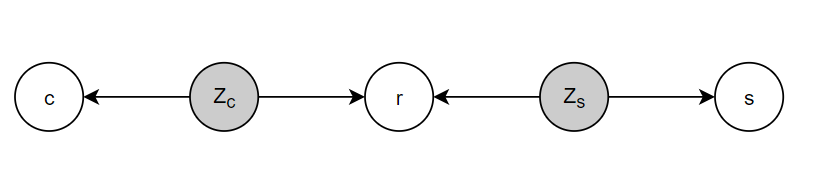
\includegraphics[height=0.9in]{gfx/f-m-m.png}\label{fig:optimierung:loesungen:abb2:1}}\\
    \subfloat[Flexible Mixture Model mit multi-kriteriellen Bewertungen und Dependency-Struktur]{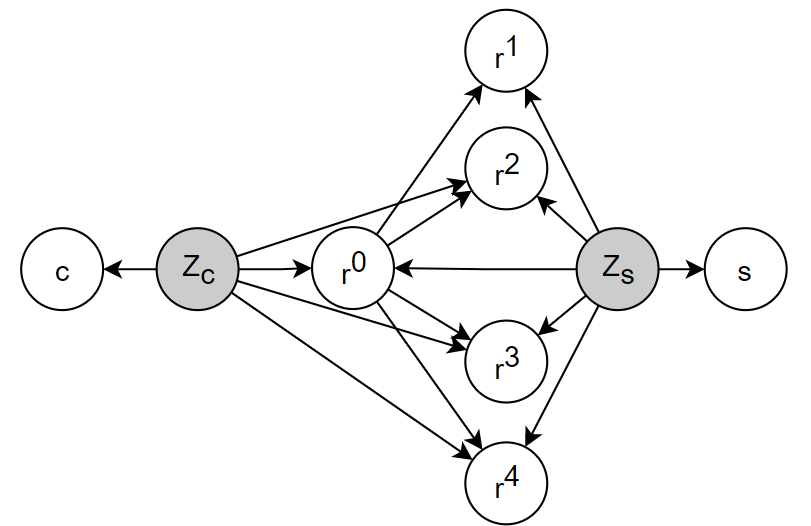
\includegraphics[height=2.20in]{gfx/f-m-m-2.png}\label{fig:optimierung:loesungen:abb2:2}}\\
  \caption[Probabilistischer Modellierungs-Ansatz]{Probabilistischer Modellierungs-Ansatz\\
	(Eigene Darstellung in Anlehnung an \cite[S. 836]{adomavicius:4:inbook})}\label{fig:optimierung:loesungen:abb2}
\end{figure}

\textcite[S. 235]{sahoo:article} erweitern das \ac{FMM} um multi-kriterielle Bewertungen.
Weiter unterstellen \textcite[S. 236f.]{sahoo:article} eine strukturelle Abhängigkeit zwischen den Bewertungen der einzelnen Kriterien (inkl. Gesamtbewertung).
Nach \textcite[S. 236f.]{sahoo:article} besteht die stärkste Abhängigkeit (durchschnittliche Korrelation) zwischen der Gesamtbewertung eines Elements und den Bewertungen der einzelnen Kriterien.
% Das bedeutet, dass nicht jedes Bewertungskriterium gänzlich neue Information über die Präferenzen eines Nutzers liefert, sondern, dass die Gesamtbewertung einen starken Einfluss auf die Ausprägung der Bewertungen der einzelnen Kriterien hat \cite[S. 235]{sahoo:article}.
Die Abhängigkeiten (engl.: Dependency Structure) zwischen den Kriterien bilden \textcite[S. 235]{sahoo:article} in Anlehnung an Dependence Trees von \textcite[S. 463]{chow:article} als Baum ab.
Die Integration multi-kriterieller Bewertungen in das ursprüngliche \ac{FMM} in Form einer der Dependency Structure ist in Abbildung \ref{fig:optimierung:loesungen:abb2:2} grafisch dargestellt.

Die Vorhersage fehlender Bewertungen anhand des Ansatzes erfolgt in zwei Schritten. 
Im ersten Schritt werden die Parameter ($Z_{c}$ und $Z_{s}$ \cite[S. 4]{si:inproceedings}) des \ac{FMM} mithilfe des Expectation Maximization Algorithmus von \textcite[S. 1ff.]{dempster:article} bestimmt \cite[S. 863]{adomavicius:4:inbook}.
Unter Anwendung der Parameter wird darauffolgend der Wert einer fehlenden Bewertung als die Bewertung mit der höchsten Wahrscheinlichkeit vorhergesagt \cite[S. 863]{adomavicius:4:inbook}. 
% HIER WEITERMACHEN mit Erklärung der Vorgehensweise zur Bestimmung fehlender Bewertungen

% Wenn im bereich multi-criteria ratings, dann unterscheiden zwischen vorhandenes overall rating ode rnicht vorhandenes overall rating
% wenn bei overall rating können ansätze aus der allgemeinen multi-kriteriellen optimierung auf RS übertragen werden

\subsection{Pareto-Optimierung}
% Skyline querie siehe Lee and Teng 2007: . Incorporating multi-criteria ratings in recommendation systems.

\subsection{Aggregation}

\subsection{Bedingungen}

\shorthandon{"}